\section{Metodologia}

\subsection{Visão Geral e Arquitetura do Sistema}

O sistema foi concebido para transformar a corrida em uma experiência de sobrevivência. O usuário tenta fugir de uma horda virtual de zumbis, e a posição do personagem no jogo é determinada pela distância percorrida, pelo ritmo de corrida e por sinais biométricos. Esses elementos compõem um fluxo em que a corrida física é traduzida em uma mecânica gamificada de perseguição e fuga.

O sistema foi estruturado em três componentes principais: relógio, aplicativo móvel e \textit{backend}. O relógio atua como fonte de frequência cardíaca, enviada ao aplicativo por mensagens do \textit{Wear OS}, o sistema operacional para relógios inteligentes do ecossistema Android \cite{androidWearMessageClient}. O aplicativo móvel é responsável pela autenticação do usuário, seleção da horda de zumbis, coleta de localização e aceleração, recepção do BPM (batimentos por minuto), envio periódico da telemetria e renderização da corrida gamificada. O \textit{backend}, ou servidor, mantém a sessão online como fonte de verdade, calcula o estado da corrida, atualiza o \textit{ranking} e persiste os dados duráveis.

Neste trabalho, sessão de treino é o ciclo iniciado quando o usuário autenticado cria uma corrida pelo \textit{endpoint} REST (\textit{Representational State Transfer}) \texttt{POST /sessions/start}. A sessão pode ser associada a uma horda e a uma distância-alvo. Ao ser criada, ela gera um registro relacional de treino e inicializa no Redis o estado temporário usado durante a corrida. No aplicativo, a sessão remota pode estar em estados como \texttt{IDLE}, \texttt{STARTING}, \texttt{CONNECTING}, \texttt{ACTIVE}, \texttt{ENDING} e \texttt{ERROR}. No \textit{backend}, o estado lógico da corrida é publicado como \texttt{RUNNING}, \texttt{CAUGHT} ou \texttt{ESCAPED}. O encerramento normal ocorre por \texttt{/sessions/\{sessionId\}/finish}; em falha de conexão, o aplicativo desconecta o \textit{WebSocket}, limpa a sessão ativa e registra erro local, sem fila de reenvio ou retomada automática.

A implementação móvel utiliza \textit{Kotlin Multiplatform} e \textit{Compose Multiplatform} para compartilhar interface, modelos e contratos de comunicação. O Android é a plataforma funcional de referência, pois concentra sensores, \textit{Wear OS}, serviço em primeiro plano e renderização com KorGE, um motor de jogos multiplataforma desenvolvido em Kotlin \cite{korgeGameEngine}. O alvo iOS existe como invólucro SwiftUI do módulo Kotlin, mas ainda não possui paridade com o fluxo Android de telemetria, sessão online e renderização. No servidor, Spring Boot 3.4.4 com Kotlin 2.1.20 foi adotado pela integração com o ecossistema JVM (\textit{Java Virtual Machine}), suporte a APIs HTTP, segurança, JPA (\textit{Java Persistence API}), WebSocket e documentação OpenAPI.

\begin{figure*}[t]
    \centering
    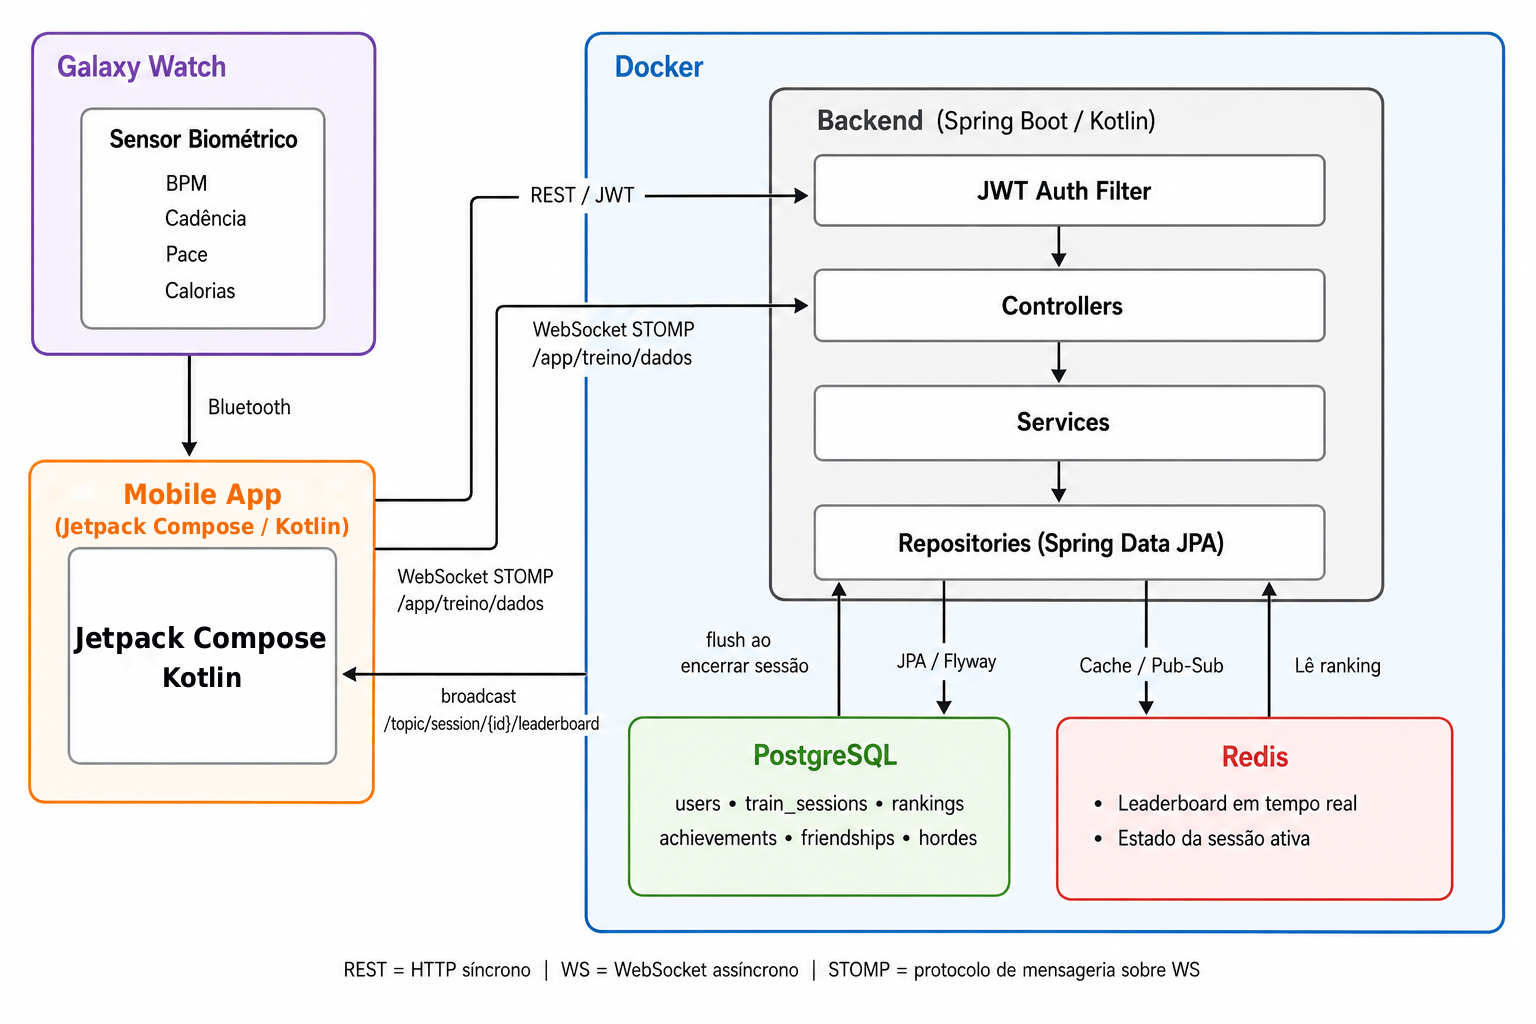
\includegraphics[width=0.9\textwidth]{figuras/diagrama_jetpack_compose_kotlin.png}
    \captionsetup{justification=centering}
    \caption{Arquitetura geral do sistema e comunicação entre o relógio, o aplicativo móvel e o backend}
    \label{fig:diagrama_de_blocos}
\end{figure*}

\subsection{Aplicativo Móvel e Coleta de Telemetria}

No Android, a telemetria combina localização, aceleração e frequência cardíaca. A localização é obtida pela API de localização combinada do Google Play Services, e a aceleração é lida a partir dos sensores de movimento da plataforma Android \cite{googleFusedLocationProvider, androidLocationUpdates, androidMotionSensors}. O BPM é recebido do relógio por mensagens \textit{Wear OS} no \textit{endpoint} \texttt{/telemetry} \cite{androidWearMessageClient, googleWearableListenerService}. Esses dados são centralizados em um repositório de telemetria, que disponibiliza um fluxo de estado observado pela interface e pela sessão online.

O estado de telemetria mantém a sessão local de movimento, a última localização, a última aceleração, a última amostra biométrica, a estratégia de coleta em uso e eventuais problemas de disponibilidade. A estratégia alterna entre movimento isolado e movimento com BPM de acordo com a conexão do relógio e a disponibilidade de frequência cardíaca. Durante uma sessão online, o aplicativo converte esse estado em uma mensagem biométrica compatível com o contrato do servidor, incluindo dados de identificação, tempo, frequência cardíaca, velocidade, ritmo, distância acumulada e campos opcionais de rastreamento de latência.

O envio ao \textit{backend} é limitado a uma mensagem por segundo, reduzindo o volume de comunicação e mantendo atualizações periódicas do estado da corrida. A interface é construída em \textit{Compose Multiplatform} e apresenta autenticação, seleção de horda, corrida, \textit{ranking}, perfil, permissões e histórico. A cena da corrida é renderizada com KorGE no Android. Em sessão online, ela apenas representa visualmente o estado recebido do servidor, sem calcular de forma independente o resultado da corrida.

Como a coleta depende de localização, movimento e execução contínua, o aplicativo Android verifica permissões, provedor de localização, sensor de movimento, conectividade e permissão de notificação quando exigida \cite{androidLocationPermissions, androidLocationSettings}. Durante a corrida, um serviço em primeiro plano mantém a coleta ativa e exibe notificação persistente, prática alinhada ao tipo de execução contínua prevista pela plataforma Android \cite{androidForegroundServices, androidForegroundServiceTypes}. A suíte do aplicativo contém testes para contratos HTTP, cliente STOMP, estados de sessão remota, mapeamento de telemetria, conversão do estado remoto para a representação visual, configuração de hordas e componentes de interface. A versão atual não possui validação integrada com sensores físicos, relógio e servidor real no mesmo cenário automatizado.

\subsection{Backend e Persistência}

O \textit{backend} organiza controladores REST, controlador WebSocket, serviços de negócio, serviços Redis, entidades JPA e repositórios. Os \textit{endpoints} REST são usados para autenticação, usuários, hordas, criação e encerramento de sessões, \textit{ranking} da sessão e \textit{ranking} global. A autenticação HTTP é \textit{stateless} (não mantém estado de sessão no servidor e baseada em JWT (\textit{JSON Web Token}), os \textit{tokens} são assinados com chave HMAC-SHA pela biblioteca JJWT, e as senhas são armazenadas com BCrypt. O \textit{endpoint} WebSocket \texttt{/ws} permanece liberado na configuração HTTP atual.

A persistência combina PostgreSQL e Redis com finalidades distintas. O PostgreSQL armazena dados duráveis, como usuários, sessões de treino, hordas, \textit{rankings}, conquistas, amizades e amostras biométricas. A entidade \texttt{BiometricData} registra amostras recebidas durante a sessão de forma assíncrona, contendo informações como tempo, BPM, velocidade, ritmo, distância acumulada e vínculo com a sessão. Portanto, a versão atual realiza gravações no PostgreSQL durante a corrida, embora o estado em tempo real da sessão seja mantido no Redis.

No Redis, a sessão mantém o \textit{ranking} temporário em ZSET, o instante inicial, o ritmo da horda, a indicação de horda adaptativa, a distância-alvo, o conjunto de sessões ativas e o estado biométrico instantâneo de cada usuário em Hash. O TTL (\textit{time to live}) limita a permanência desses dados: durante a sessão, as chaves recebem expiração de 24 horas. Após o encerramento, as chaves específicas da sessão passam a expirar em uma hora. No encerramento, o servidor lê o \textit{ranking} final do Redis, grava os registros de \texttt{Ranking}, atualiza a distância total da \texttt{TrainSession}, incrementa o \textit{ranking} global mensal e executa verificações de conquistas e notificações.

A infraestrutura de execução é descrita pelo Docker Compose, com API, PostgreSQL, Redis e Jenkins. A integração contínua utiliza Jenkins para construir o projeto, executar testes, gerar relatórios JaCoCo e empacotar a aplicação. A suíte automatizada do \textit{backend} cobre autenticação, filtro JWT, controladores, serviços, repositórios, cálculo da horda, zonas cardíacas, persistência biométrica, \textit{ranking} e operações Redis.

\subsection{Comunicação em Tempo Real}

O fluxo de comunicação em tempo real segue a sequência relógio, aplicativo móvel, \textit{backend}, aplicativo móvel e relógio. O relógio envia BPM ao aplicativo pelo caminho Wear OS \texttt{/telemetry} \cite{androidWearMessageClient}. O aplicativo usa REST (Representational State Transfer) para operações discretas, como autenticação, carregamento de hordas, criação da sessão e encerramento. Após a criação da sessão, o aplicativo abre conexão em \texttt{/ws}, envia telemetria ao destino STOMP (\textit{Simple Text Oriented Messaging Protocol}) \texttt{/app/train/data} e assina os tópicos \texttt{/topic/session/\{sessionId\}/leaderboard} e \texttt{/topic/session/\{sessionId\}/game-state}.

O tópico de \textit{ranking} publica a classificação da sessão, a posição virtual da horda e as zonas cardíacas dos participantes retornados pelo \textit{ranking}. O tópico de estado do jogo publica a posição do usuário, a posição da horda, a distância até a meta, a distância relativa entre o usuário e a horda, as velocidades, o progresso percentual, o estado da corrida e os campos de rastreamento de latência. O aplicativo também pode enviar ao relógio o progresso local pelo caminho \texttt{/game-progress}, incluindo distância, meta, progresso, BPM, risco, pressão da horda e resultado visual.

\subsection{Mecânica de Gamificação}

A gamificação foi modelada como uma corrida de fuga. O usuário vence quando atinge a distância-alvo antes de ser alcançado, perde quando a horda alcança ou ultrapassa sua posição após o atraso inicial. A posição do usuário é a distância acumulada enviada pelo aplicativo. A posição da horda é calculada no servidor a partir do instante inicial da sessão, de um atraso inicial de sete segundos e do ritmo configurado em minutos por quilômetro. O ritmo efetivo vem do valor definido na horda, da horda pai ou dos padrões por dificuldade: \texttt{EASY} com 10,0 min/km, \texttt{MEDIUM} com 8,0 min/km e \texttt{HARD} com 4,0 min/km.

O \textit{backend} é a fonte de verdade da corrida online. A cada mensagem biométrica válida, ele atualiza o estado instantâneo do usuário no Redis, atualiza sua distância no \textit{ranking}, calcula a posição virtual da horda e publica o novo estado do jogo. O aplicativo móvel não decide vitória ou derrota em sessão online, ele renderiza visualmente o estado recebido, ajustando corredor, horda, pressão, progresso e resultado.

O BPM é usado na versão atual como dado de \textit{biofeedback} para coleta, transmissão, persistência e cálculo de zona cardíaca quando a frequência cardíaca máxima do usuário está disponível. Ele não altera diretamente o ritmo da horda, a distância-alvo, a velocidade virtual ou a dificuldade da sessão. Assim, a adaptação implementada não deve ser descrita como ajuste cardiovascular de dificuldade.

As hordas marcadas com \texttt{isAdaptive} possuem adaptação baseada no desempenho de movimento dos participantes. O valor inicial do ritmo é gravado no Redis ao iniciar a sessão. Em cada mensagem biométrica processada, se a horda da sessão for adaptativa, o servidor considera os usuários presentes nas entradas publicadas do \textit{ranking} da sessão, calcula a média dos ritmos válidos maiores que zero e grava esse novo ritmo em \texttt{session:\{sessionId\}:horde:pace}. Se não houver ritmo válido, o valor não é atualizado. O código atual não aplica limites mínimo e máximo nem mecanismo de suavização. A atualização ocorre enquanto chegam mensagens biométricas válidas.

\subsection{Procedimentos de Avaliação}

\subsubsection{Avaliação Funcional}

A avaliação funcional foi definida a partir dos fluxos implementados e dos testes automatizados existentes. O ambiente previsto é a execução local ou em integração contínua das suítes do \textit{backend} e do aplicativo móvel, com H2 para testes relacionais do \textit{backend} e Redis disponível para os testes que dependem dele. O critério de aprovação é a execução dos cenários sem falhas e a compatibilidade entre contratos móveis e \textit{endpoints} do servidor.

\begin{table}[htbp]
\centering
\caption{Cenários da avaliação funcional}
\label{tab:avaliacao_funcional}
\begin{adjustbox}{max width=\columnwidth}
\begin{tabular}{p{2.2cm}p{2.8cm}p{2.8cm}}
\hline
    \textbf{Funcionalidade} & \textbf{Cenário} & \textbf{Resultado esperado} \\ \hline
    Autenticação & Cadastro, login e validação de JWT & Token aceito em rotas protegidas e senha armazenada com BCrypt. \\
    Sessão online & Criação, atualização por telemetria e encerramento & Sessão criada, estado Redis atualizado e dados finais persistidos. \\
    Gamificação & Comparação entre usuário, horda e distância-alvo & Estados \texttt{RUNNING}, \texttt{CAUGHT} e \texttt{ESCAPED} coerentes. \\
    Aplicativo móvel & Mapeamento de telemetria e mensagens remotas & Contratos enviados e recebidos compatíveis com o backend. \\ \hline
    \end{tabular}
    \end{adjustbox}
\end{table}

\subsubsection{Avaliação de Latência}

A avaliação de latência foi preparada no código por meio dos campos \texttt{latencyTraceId}, \texttt{clientSentAtElapsedMs} e \texttt{backendProcessingMs}. O ponto inicial é o envio da mensagem biométrica pelo aplicativo móvel, o ponto final é o recebimento pelo aplicativo do estado do jogo associado ao mesmo identificador de rastreamento. O \textit{backend} registra o tempo interno de processamento e devolve esse valor na resposta do tópico \texttt{/topic/session/\{sessionId\}/game-state}. As métricas previstas são quantidade de amostras, média, mediana, percentil 95, máximo e tratamento separado de amostras sem correspondência entre envio e resposta.

\subsubsection{Avaliação de Usabilidade}

A avaliação de usabilidade foi planejada para analisar a interação do usuário com os fluxos centrais da aplicação, como autenticação, seleção de hordas, início da corrida, acompanhamento da sessão e sincronização de dados. O procedimento foi estruturado a partir da observação de uso prático dos dispositivos, considerando o impacto das restrições de tela e processamento do \textit{smartwatch}. As métricas qualitativas previstas concentram-se na clareza dos indicadores visuais de estado, na percepção da proposta gamificada e na facilidade de uso do relógio inteligente como dispositivo complementar.
